\documentclass[conference]{IEEEtran}
\hyphenation{op-tical net-works semi-conduc-tor}

\usepackage{graphicx}

\begin{document}
\title{Free to Design 100 Faulty Lightbulbs}

\author{
\IEEEauthorblockN{Dean Sutton}
\IEEEauthorblockA{MetService}
}

% make the title area
\maketitle

\begin{abstract}
I propose creating a freedom system where people are free to explore, fail and then succeed. The symbolic name for this system is \emph{Freedom Fridays}. People get a day a week free from normal duties. This system will rely on supporting leadership, training, and trust to overcome the problems that plague parts of MetService. Problems include purpose (a.k.a. task) switching, fear of failure, and singular points of view.   
\end{abstract}

\section{Introduction}
Providing the support for people to fail is key to company growth. Why? before growth comes learning. Learning requires failure. Therefore, MetService must learn how to learn and deal with failure. This will involve training, but more importantly it will require leadership that embraces failure as a sign of learning.  

This proposal suggests that before training modules are developed the company first gives... Freedom 

\section{The Key Problems}
To 

\subsection{Purpose Switching}
MetService has multiple purposes. Different parts of the organisation deal with one or maybe more of those purposes. Purpose switching sometimes gets mistaken for task switching. Task switching is hard, but it gets harder when you also switch purpose. People with really high emotional quotients can deal with this. However, for the mere mortal it leads to confusion. Introverts, especially well educated ones, don't like to be confused. Confusion in combination with pressure to achieve results leads to amygdala hijacks and the inability to think objectively. This is a negative cycle. Figure \ref{fig:peoplesystems} shows the positive feedback cycle. People need to feel that they create and operate systems that produce valuable things to affirm their purpose.

\begin{figure}[!h]
\centering
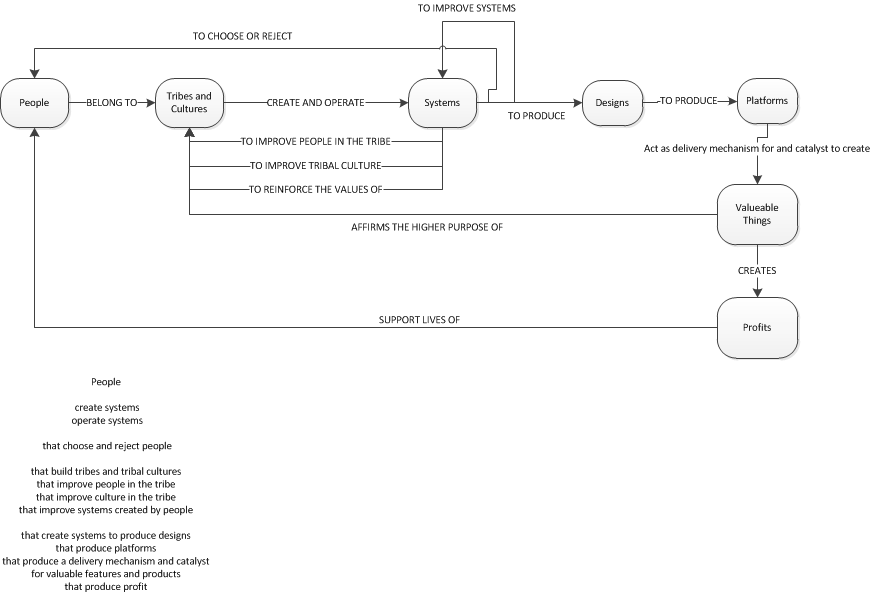
\includegraphics[width=2.5in]{SystemCreation.png}
\caption{The positive feeback cycle between tribes, people, systems and company profit. \textcopyright Grant Reid}
\label{fig:peoplesystems}
\end{figure}


\subsection{Fear of Fail}
When did I do my most learning. University. Why? I failed heaps.



\subsection{Singular Point of View}
Three objects on a table. A rugby ball, toilet paper and a gold golf ball. The objective is to take the object of most value. However, two people are chosen to decide what object to take. They both look at the objects from different perspectives. One can see the golf ball, the other can not. How does the person who sees the golf ball convince the other that it is there? This situation usually leads to fighting when there is an absense of trust. 

\section{Designing the Light Bulb}

\subsection{Freedom Fridays}

\subsubsection{Risks}

\subsection{Add Fuel To Freedom}
Present a problem, present a solution - Any team

\section{Conclusion}
The conclusion goes here.

\end{document}

